\documentclass[11pt,paper=a4]{scrartcl}

%include all used packages
\usepackage[a4paper,top=2cm,bottom=2.5cm,left=1.5cm,right=1.5cm,marginparwidth=1.75cm]{geometry}

% Language setting
\usepackage[ngerman]{babel}
% deutsche Umlaute
\usepackage[utf8]{inputenc}
\usepackage[T1]{fontenc}

\usepackage{listings}

%Schriftart
\renewcommand{\familydefault}{\sfdefault}

\usepackage[activate]{microtype}
%Abb. anstatt Abbildung
\renewcaptionname{ngerman}{\figurename}{Abb.}
\usepackage[dcucite]{harvard}
\renewcommand{\harvardand}{und}

%damit nur fref verwendet werden kann umm einen verweis auf eine Abbildung einzufügen
\newcommand{\fref}[1]{\figurename\ \ref{#1}}

%Schriftgrösse Abb. und Tabelle
\usepackage{caption}
\captionsetup[figure]{font=scriptsize}
\captionsetup[table]{font=scriptsize}

%um Tabellen farblich zu gestalten
\usepackage[table]{xcolor}

\usepackage{float}
% Useful packages
\usepackage{amsmath}
\usepackage{graphicx}
\usepackage[colorlinks=true, allcolors=black]{hyperref}
\setlength{\parindent}{0pt}
\usepackage{setspace}
%Keine Silbentrennung
% \usepackage[none]{hyphenat}
\tolerance=1
\emergencystretch=\maxdimen 
\hbadness=10000
% to use a for loop
\usepackage{pgffor}

%Tabellen mit Zeilenumbruch
\usepackage{tabulary} 
\usepackage{tabularx} 

\usepackage{scrlayer-fancyhdr}

\usepackage{pgfplots}


% Turn on the style
\pagestyle{fancy}
% Clear the footer
\fancyfoot{}
% Set the right side of the footer to be the page number
\fancyfoot[R]{Seite | \thepage}

\usepackage{pdfpages}

\definecolor{codegreen}{rgb}{0,0.6,0}
\definecolor{codegray}{rgb}{0.5,0.5,0.5}
\definecolor{backcolour}{rgb}{0.95,0.95,0.92}

% set listing for c++ codeblocks
\lstset { %
    language=C++,
    backgroundcolor=\color{black!5}, % set backgroundcolor
    basicstyle=\footnotesize,% basic font setting
    backgroundcolor=\color{backcolour},   
    commentstyle=\color{codegreen},
    keywordstyle=\color{blue},
    numberstyle=\tiny\color{codegray},
    emph={char,double,bool,String, Serial},
    emphstyle={\color{blue}},
    breakatwhitespace=false,                         
    captionpos=b,                                    
    numbers=left,                    
    numbersep=5pt,                  
    showspaces=false,                
    showstringspaces=false,
    showtabs=false,                  
    tabsize=2
}

\begin{document}
\input{ads/mainpage}
%sets the space between text and footer

\setlength{\skip\footins}{3pc plus 5pt minus 2pt}

\setlength\arrayrulewidth{1.1pt}

\pagenumbering{roman}
\newpage
\pagestyle{plain}
\setcounter{tocdepth}{3}
    \tableofcontents
\cleardoublepage

% Inhalt
\pagestyle{fancy}
\lfoot{\footnotesize \arbeit, \autorS, \autorM, {\the\year}}
\pagenumbering{arabic}
\setcounter{page}{1}

\section{Situationsanalyse}

Im Rahmen der Gruppenarbeit im Fach Embedded Systems wollen wir mit dem Arduino Nano 33 BLE Sense ein Projekt durchführen.\\
Der Arduino Nano liefert gleich mehrere verbaute Sensoren mit. Unter anderem ist auf dem Board ein 9-achsige Trägheitsmesseinheit verbaut, welche uns auf die Idee brachte, eine Drohne mit diesem Sensor zu steuern.\\
In der weiteren Analyse hat sich aber gezeigt, dass das Protokoll zum Senden an die Drohne nicht so einfach umzusetzen ist. Aus diesem Grund haben wir uns dann entschieden, eine einfache Simulation mit Unity zu erstellen, welche mit dem Arduino Nano über USB gesteuert werden kann.

\subsection{Technische Details Arduino Nano 33 BLE Sense}
Als Übersicht sind in dieser Skizze die Sensoren des Arduino Nano 33 BLE Sense dargestellt. Für unser Projekt verwenden wir nur die beiden Sensoren, das Gyroskop und den Beschleunigungssensor. Über die USB-Schnittstelle findet der Datenaustausch zwischen Computer und Arduino statt.

\vspace{2cm}
\begin{figure}[H]
  \begin{center}
    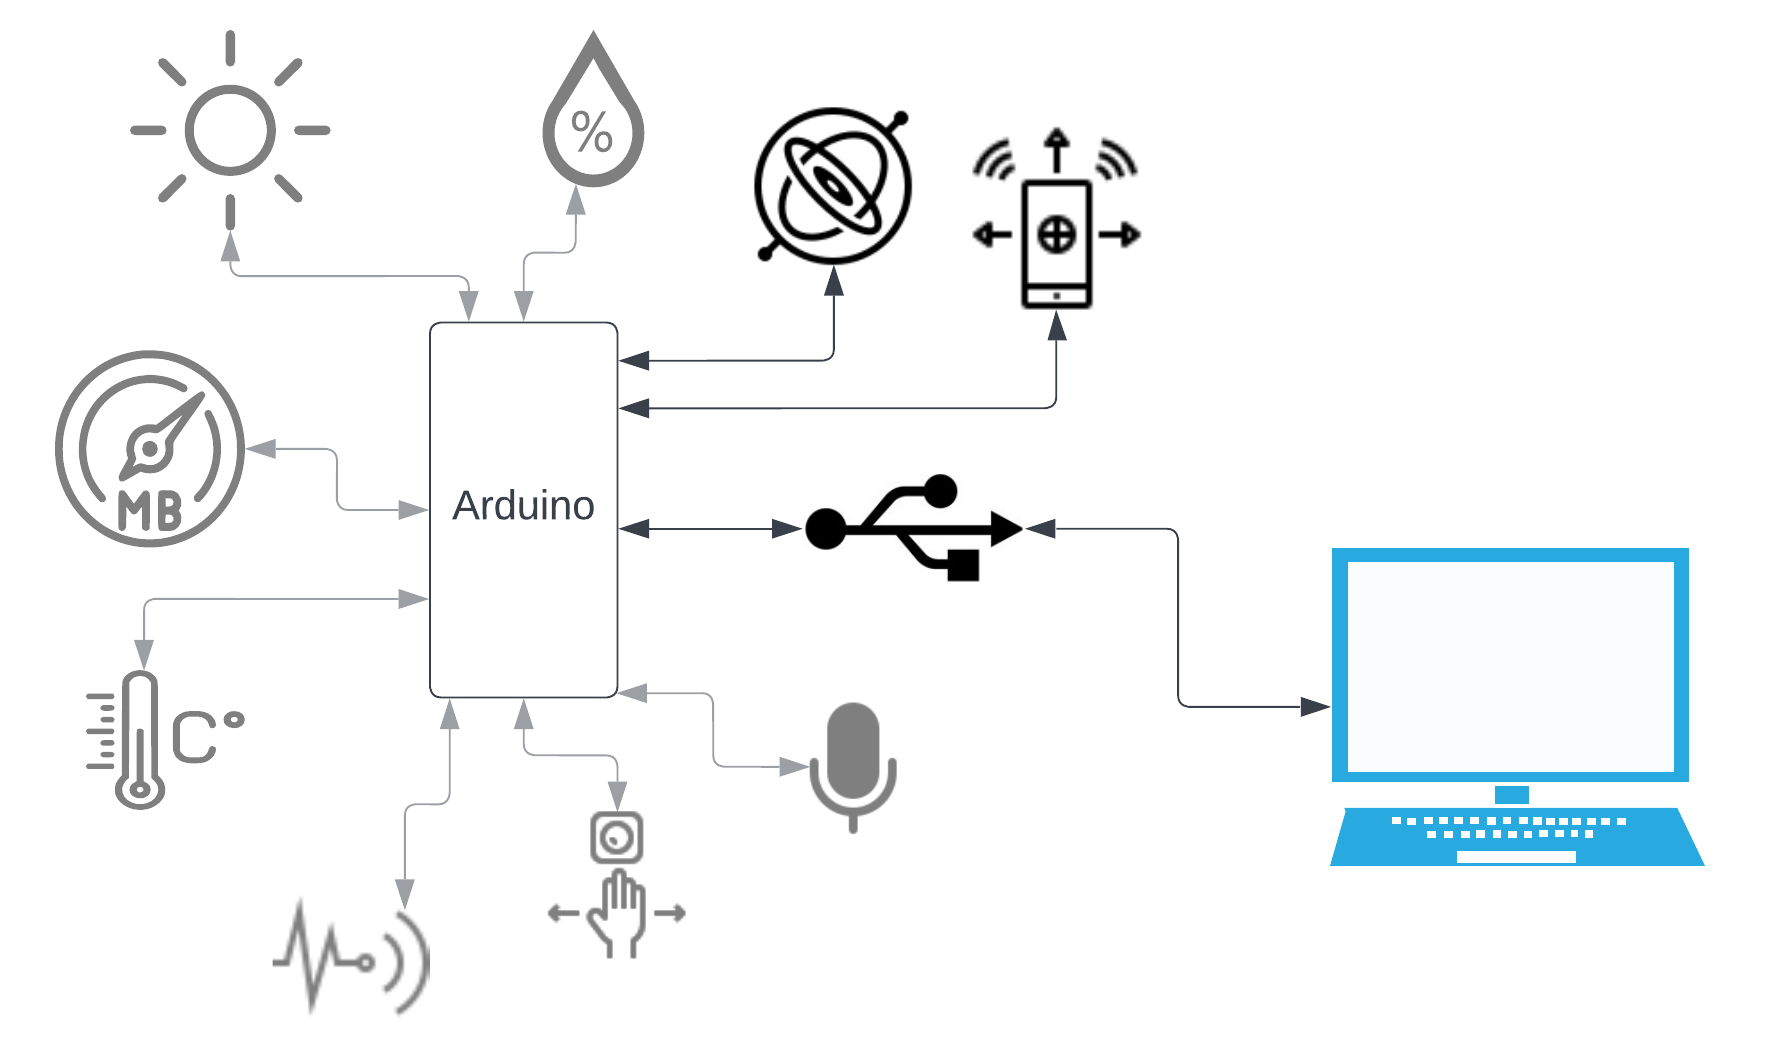
\includegraphics[width=0.6\linewidth]{content/images/system.png}
    \caption{Arduino Sensoren}
  \end{center}
\end{figure}

\newpage
Hier werden die wichtigsten Daten des Arduino Boards tabellarisch aufgelistet:

\begin{table}[H]
  \centering
  \settowidth\tymin{\textbf{MP34DT05}}
  \setlength\extrarowheight{2pt}
  \begin{tabulary}{1.0\textwidth}{|L|L|}
    \hline
    Takt &
    64Mhz\\
    \hline
    Bit & 32 \\
    \hline
    Mikrocontroller& nRF52840 \\
    \hline
    Flash & 1024KB \\
    \hline
    SRAM&  256KB\\
    \hline
    Anschlüsse& USB, I2C, SPI, Bluetooth \\
    \hline
    \textbf{LSM9DS1}& \textbf{Das LSM9DS1 ist ein System-in-Package mit einem 3D-Digital-Linearbeschleunigungssensor, ein 3D-Digital Winkelgeschwindigkeitssensor und ein digitaler 3D-Magnet Sensor.\newline
    Das LSM9DS1 hat einen linearen Beschleunigungsendwert von ± 2 g / ± 4 g / ± 8 g / ± 16 g, ein Magnetfeld mit voller Skala von ±4/±8/±12/±16 Gauss und einer Winkelgeschwindigkeit von ±245/±500/±2000 dps. } \\
    \hline
    LPS22HB& Sensor für den barometrischen Druck und die Umgebungstemperatur\newline
    Der Barometer hat eine Range von 260 bis 1260 hPa.\\
    \hline
    HTS221 & Kapazitiver Digitalsensor für relative Feuchte und Temperatur\newline
    0 bis 100\% relative Feuchte mit einer Genauigkeit von ±3.5\%rH\newline
    Der Temperatursensor misst im Range von 15 bis 40°C mit einer Genauigkeit von ±0.5°C und im Range von 0 bis 60°C mit einer Genauigkeit von ±1°C\\
    \hline
    APDS-9960& Digitaler Näherungs-, Umgebungslicht-, RGB- und Gestensensor \\
    \hline
    MP34DT05& Digitales Mikrofon, z.B. für Spracherkennung \\
    \hline
  \end{tabulary}
  \caption{Technische Details}
\end{table}

\newpage
\section{Konzept}

\begin{figure}[H]
  \begin{center}
    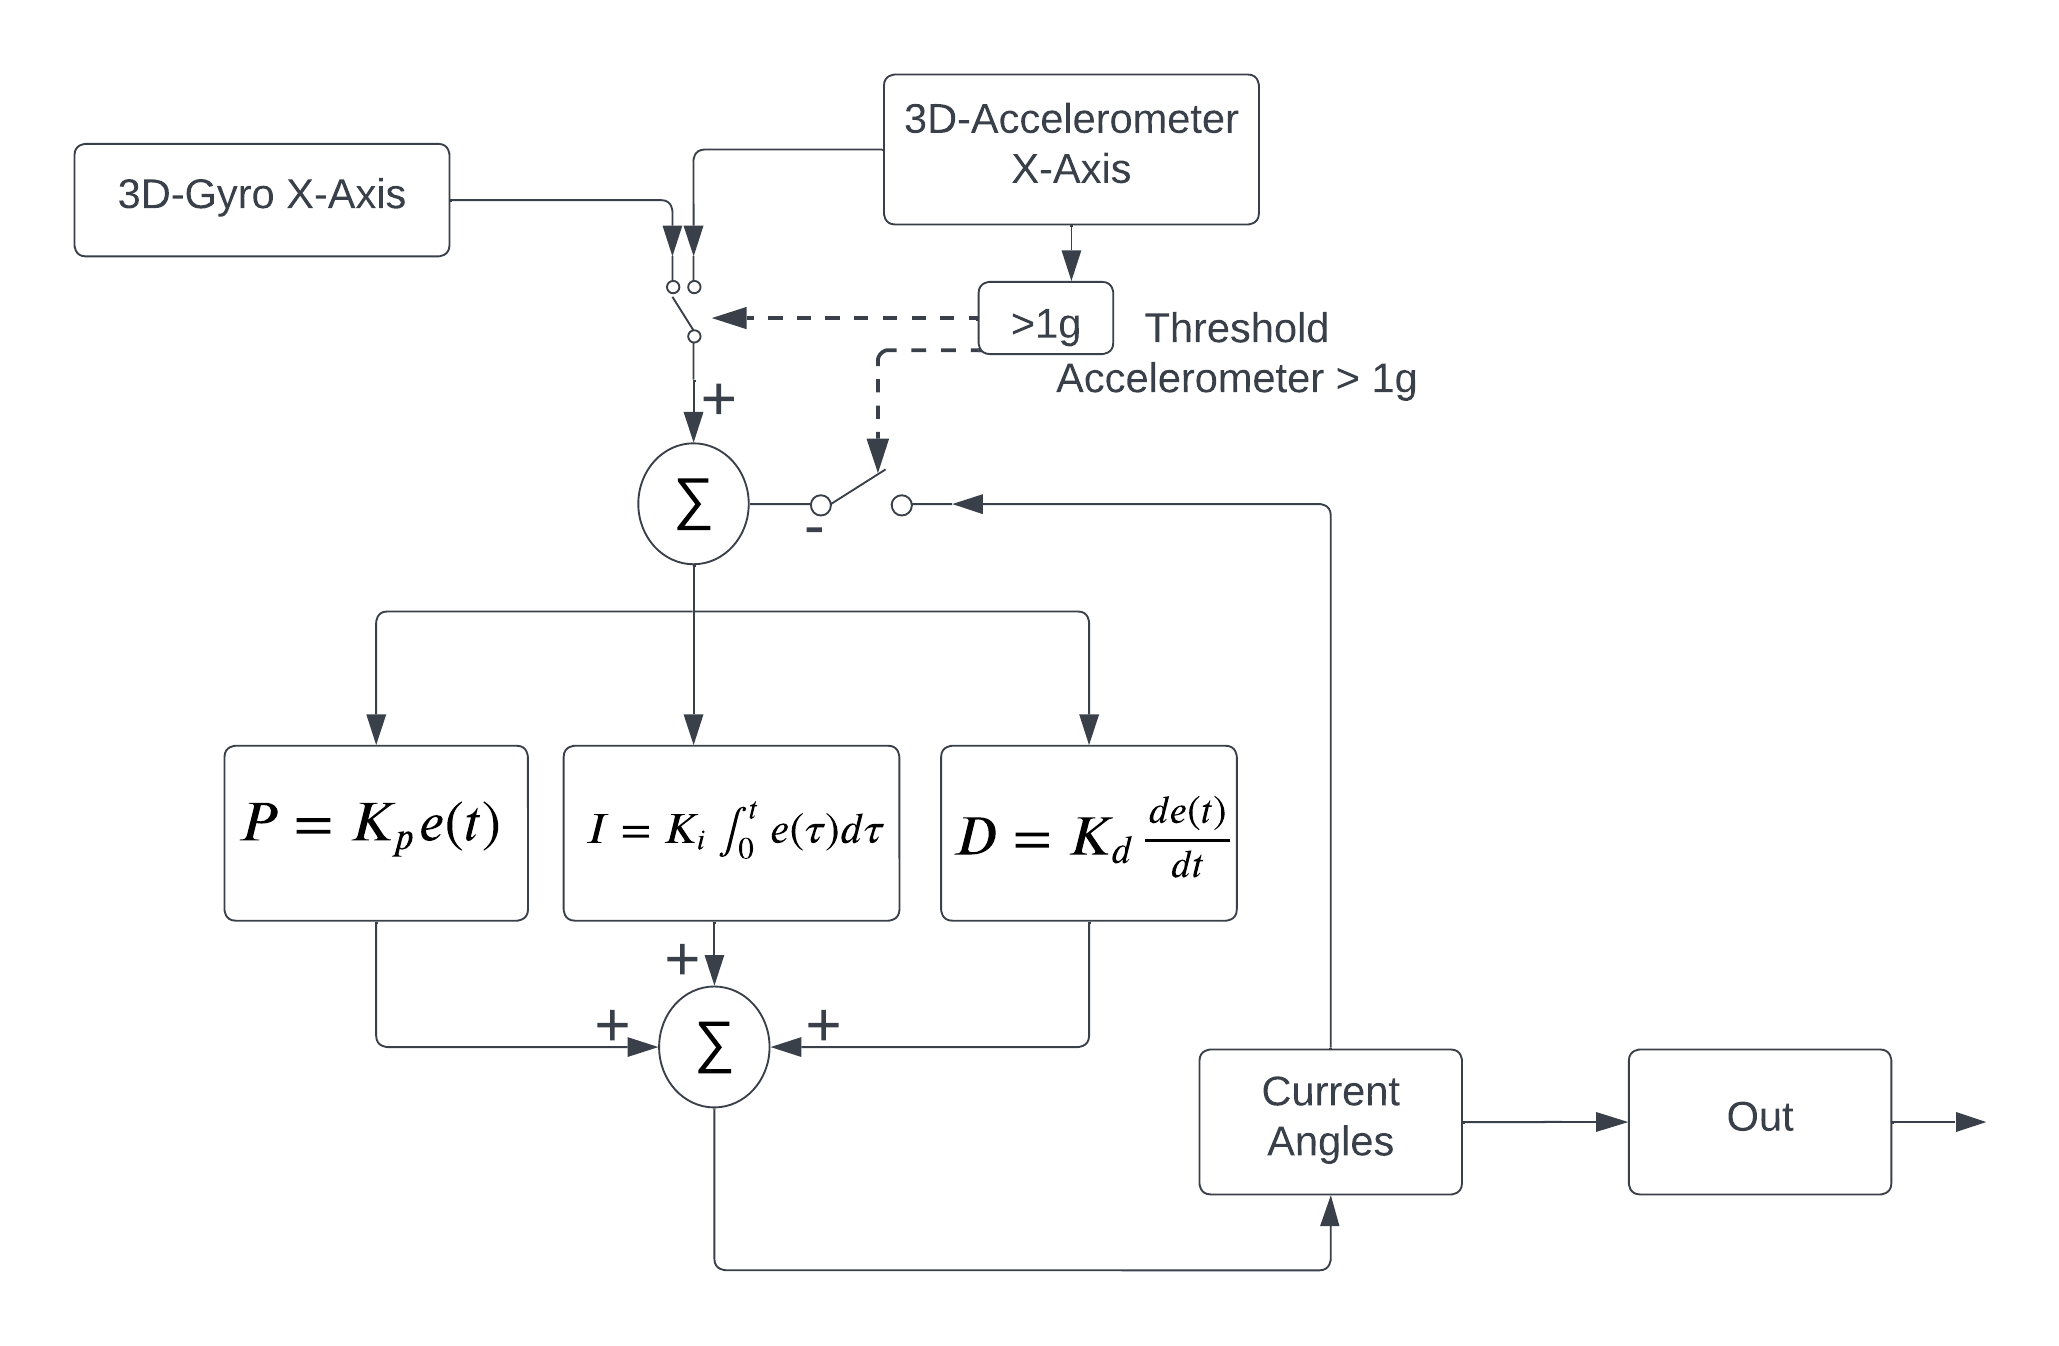
\includegraphics[width=1\linewidth]{content/images/PID_Loop.png}
    \caption{PID Loop}
  \end{center}
\end{figure}

\subsection{UseCase}
\begin{figure}[H]
  \begin{center}
    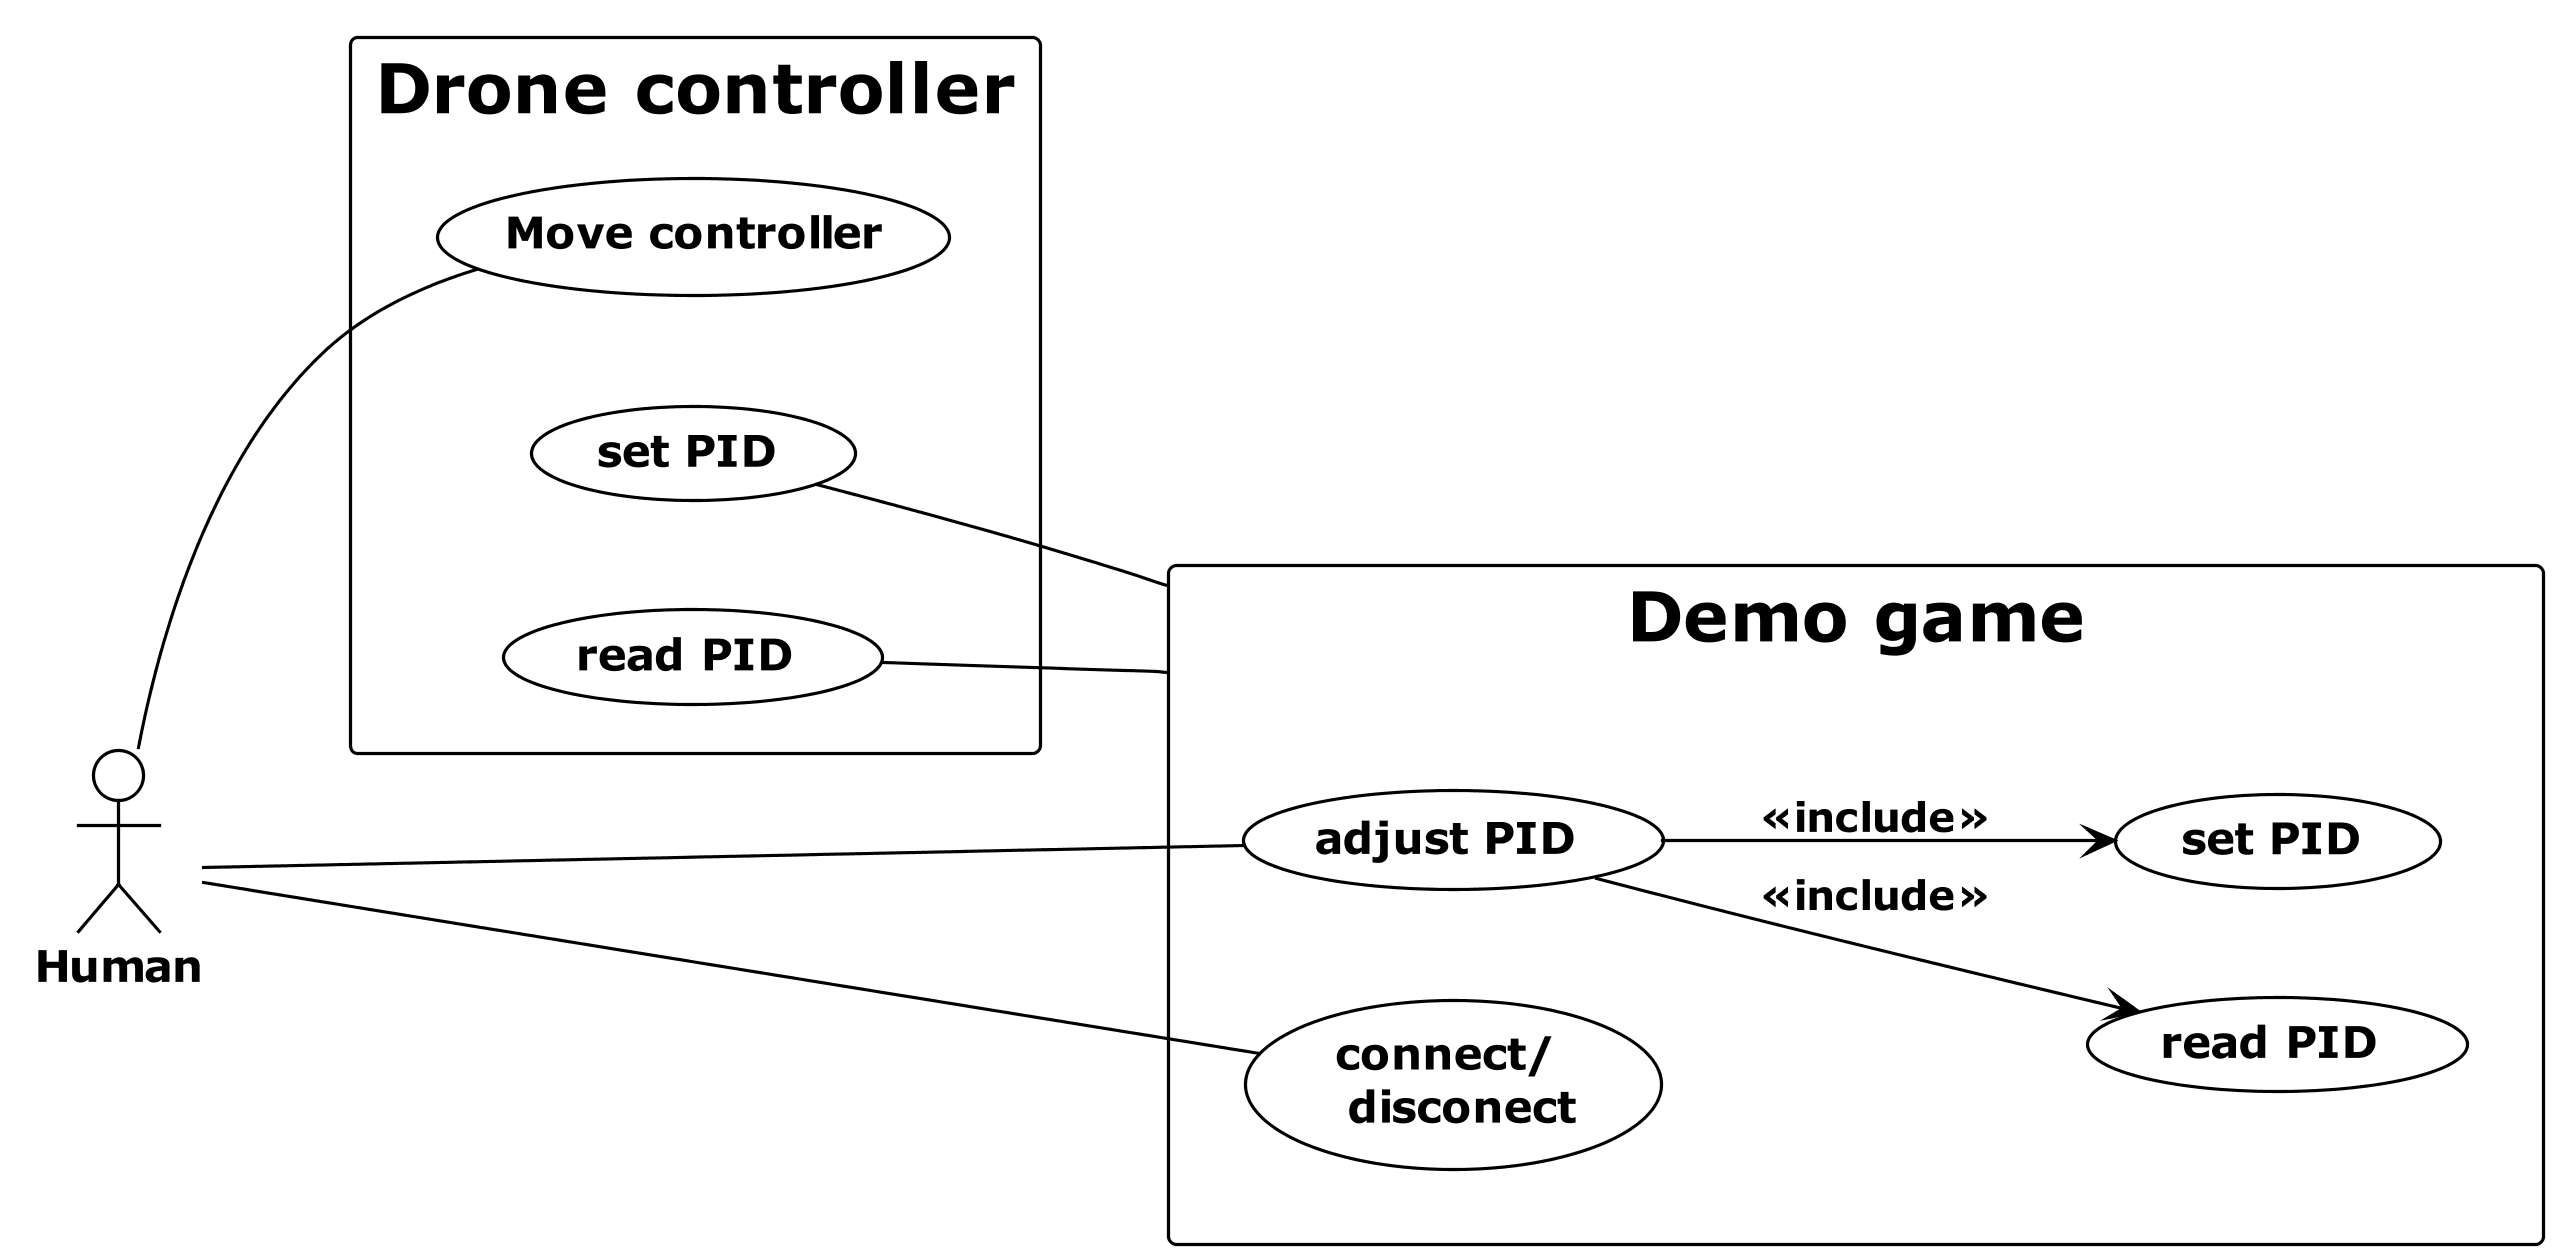
\includegraphics[width=0.8\linewidth]{content/diagrams/out/usecase/sendAngles.png}
    \caption{Send angles}
  \end{center}
\end{figure}

\subsection{Sequenzdiagramme}
\begin{figure}[H]
  \begin{center}
    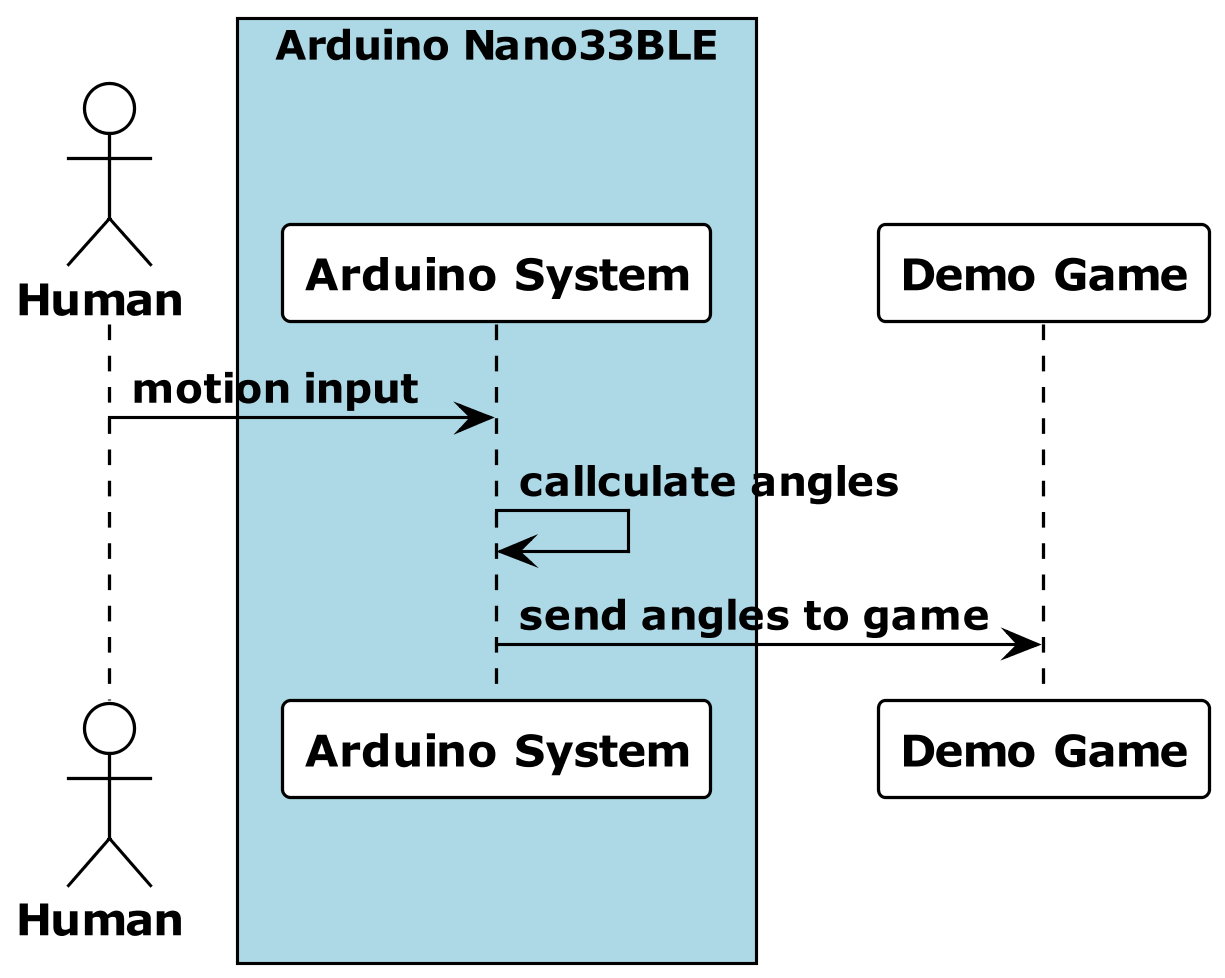
\includegraphics[width=0.7\linewidth]{content/diagrams/out/sequence/system.png}
    \caption{System}
  \end{center}
\end{figure}

\begin{figure}[H]
  \begin{center}
    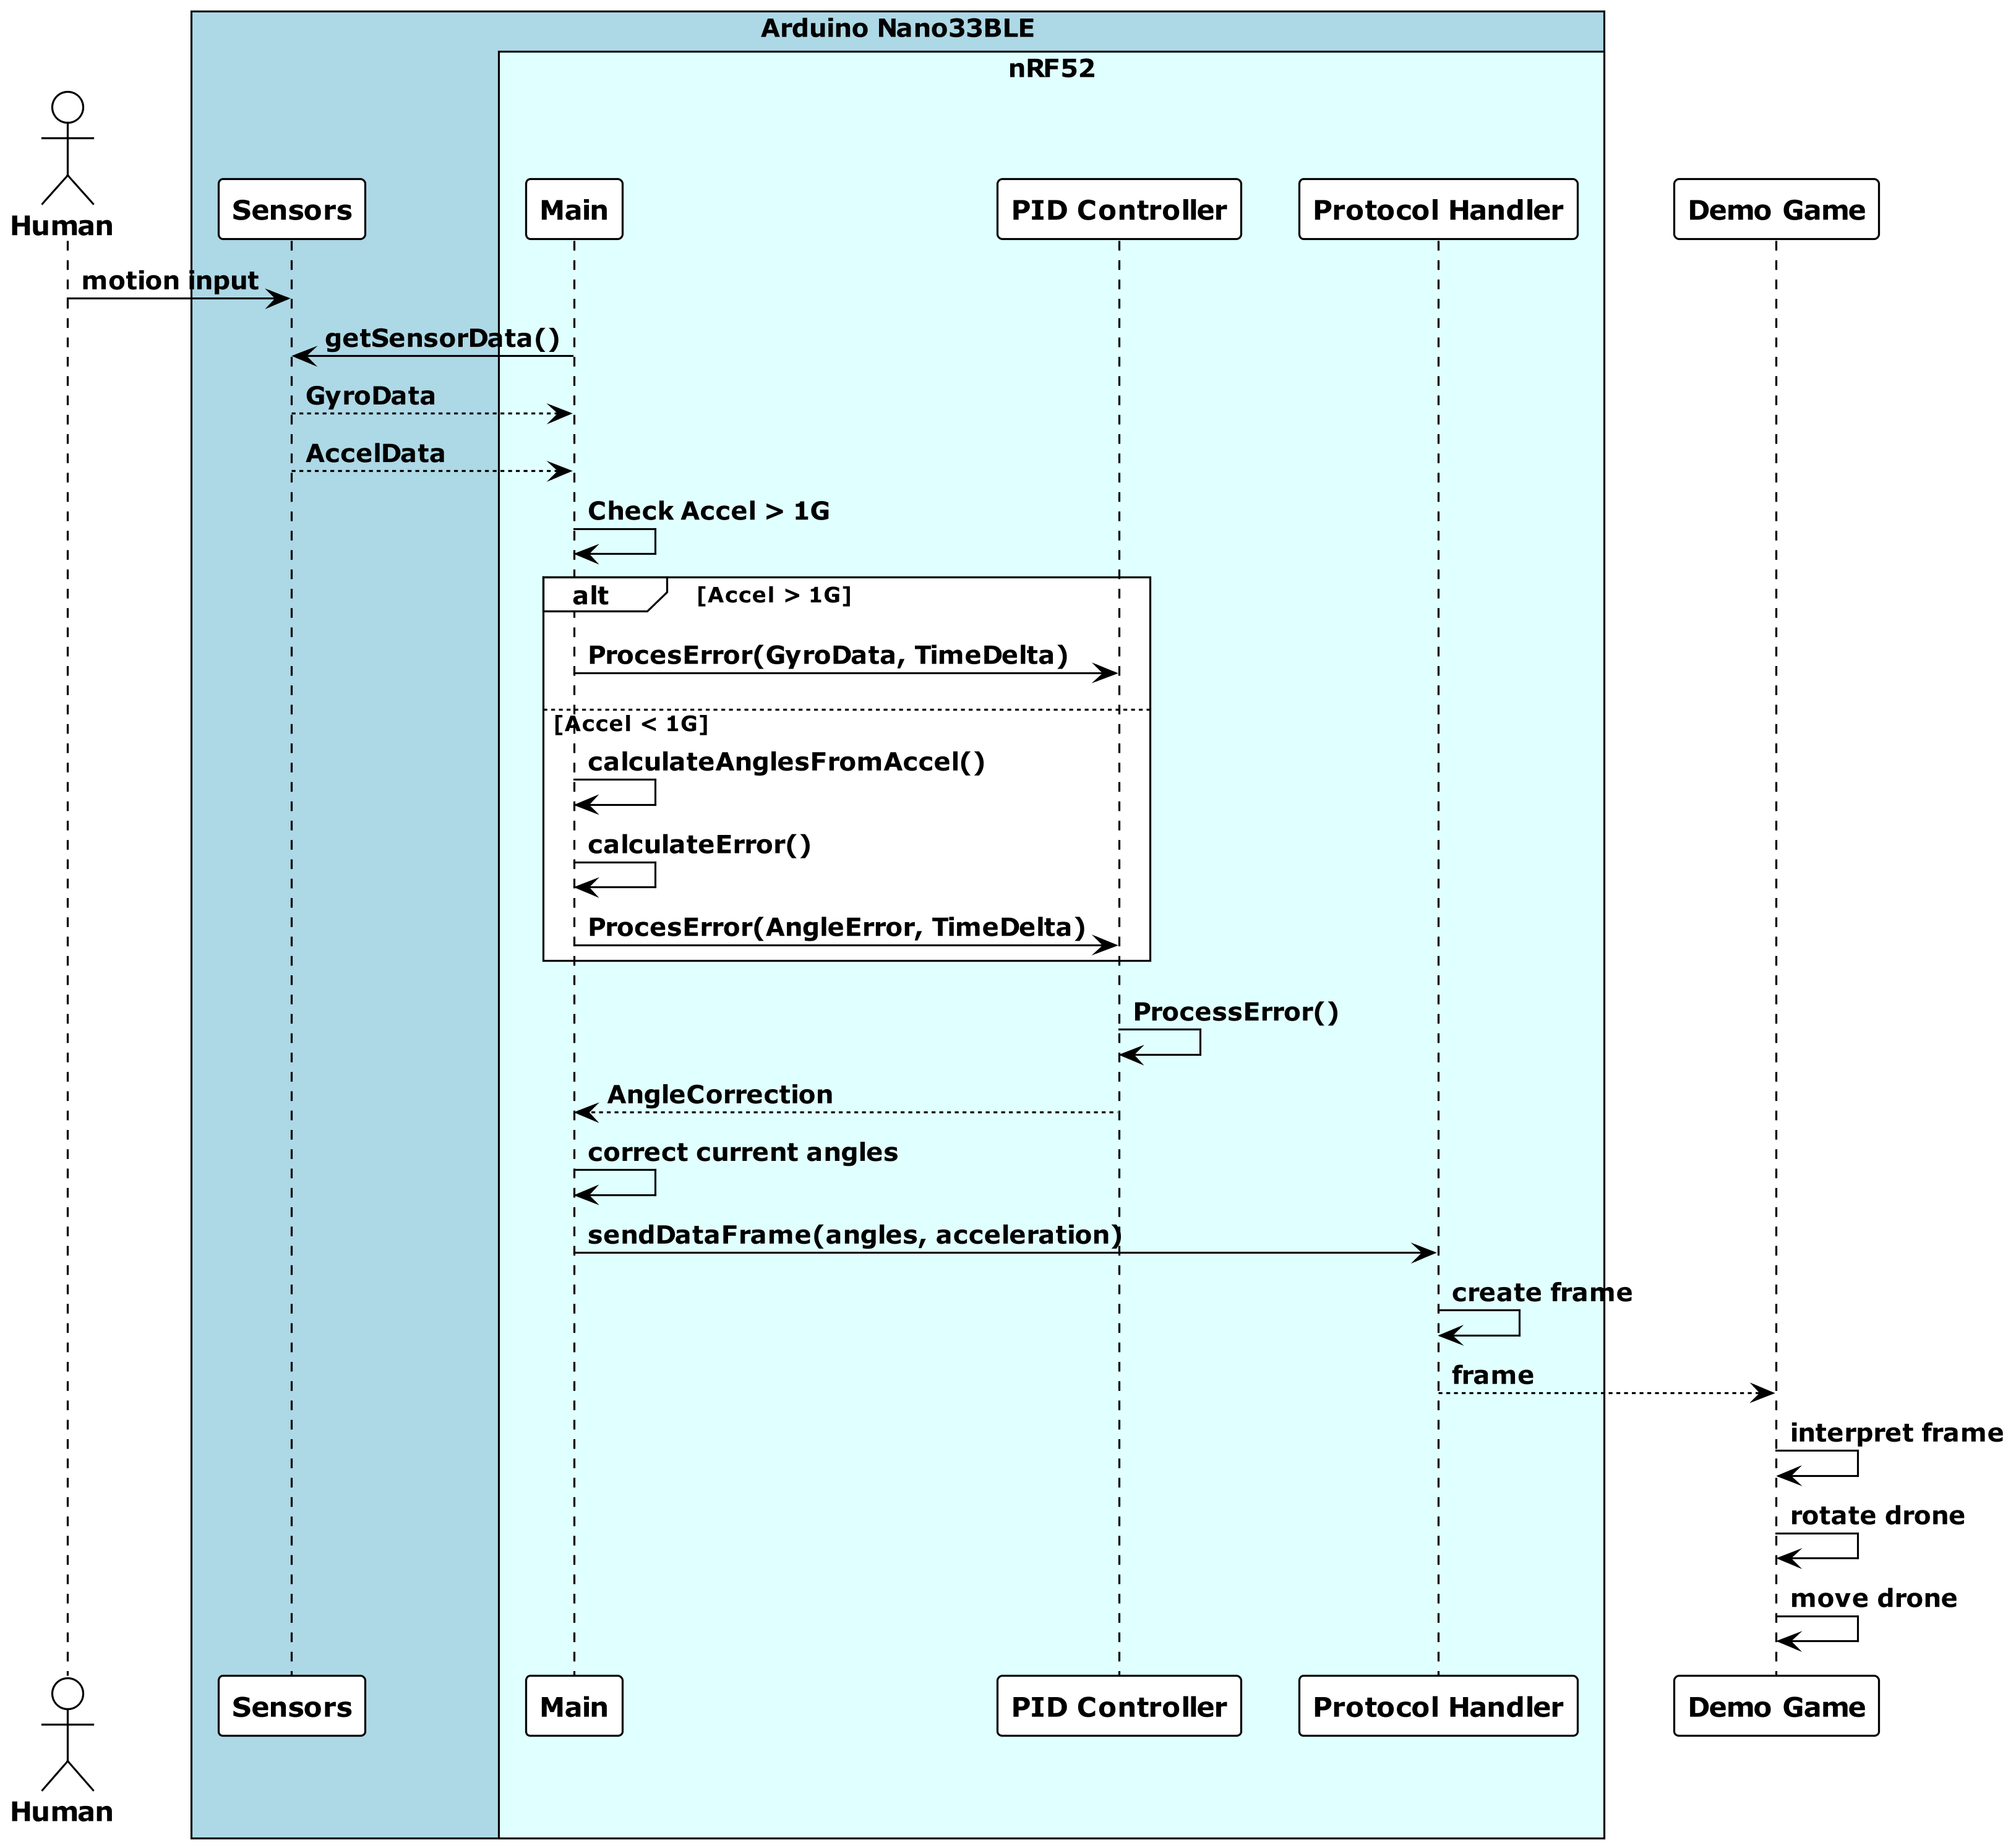
\includegraphics[width=0.8\textheight]{content/diagrams/out/sequence/moveController.png}
    \caption{Move controller}
  \end{center}
\end{figure}


\section{Implementation}
Kaptitel beschreibt die implementation

\begin{figure}[H]
  \begin{center}
    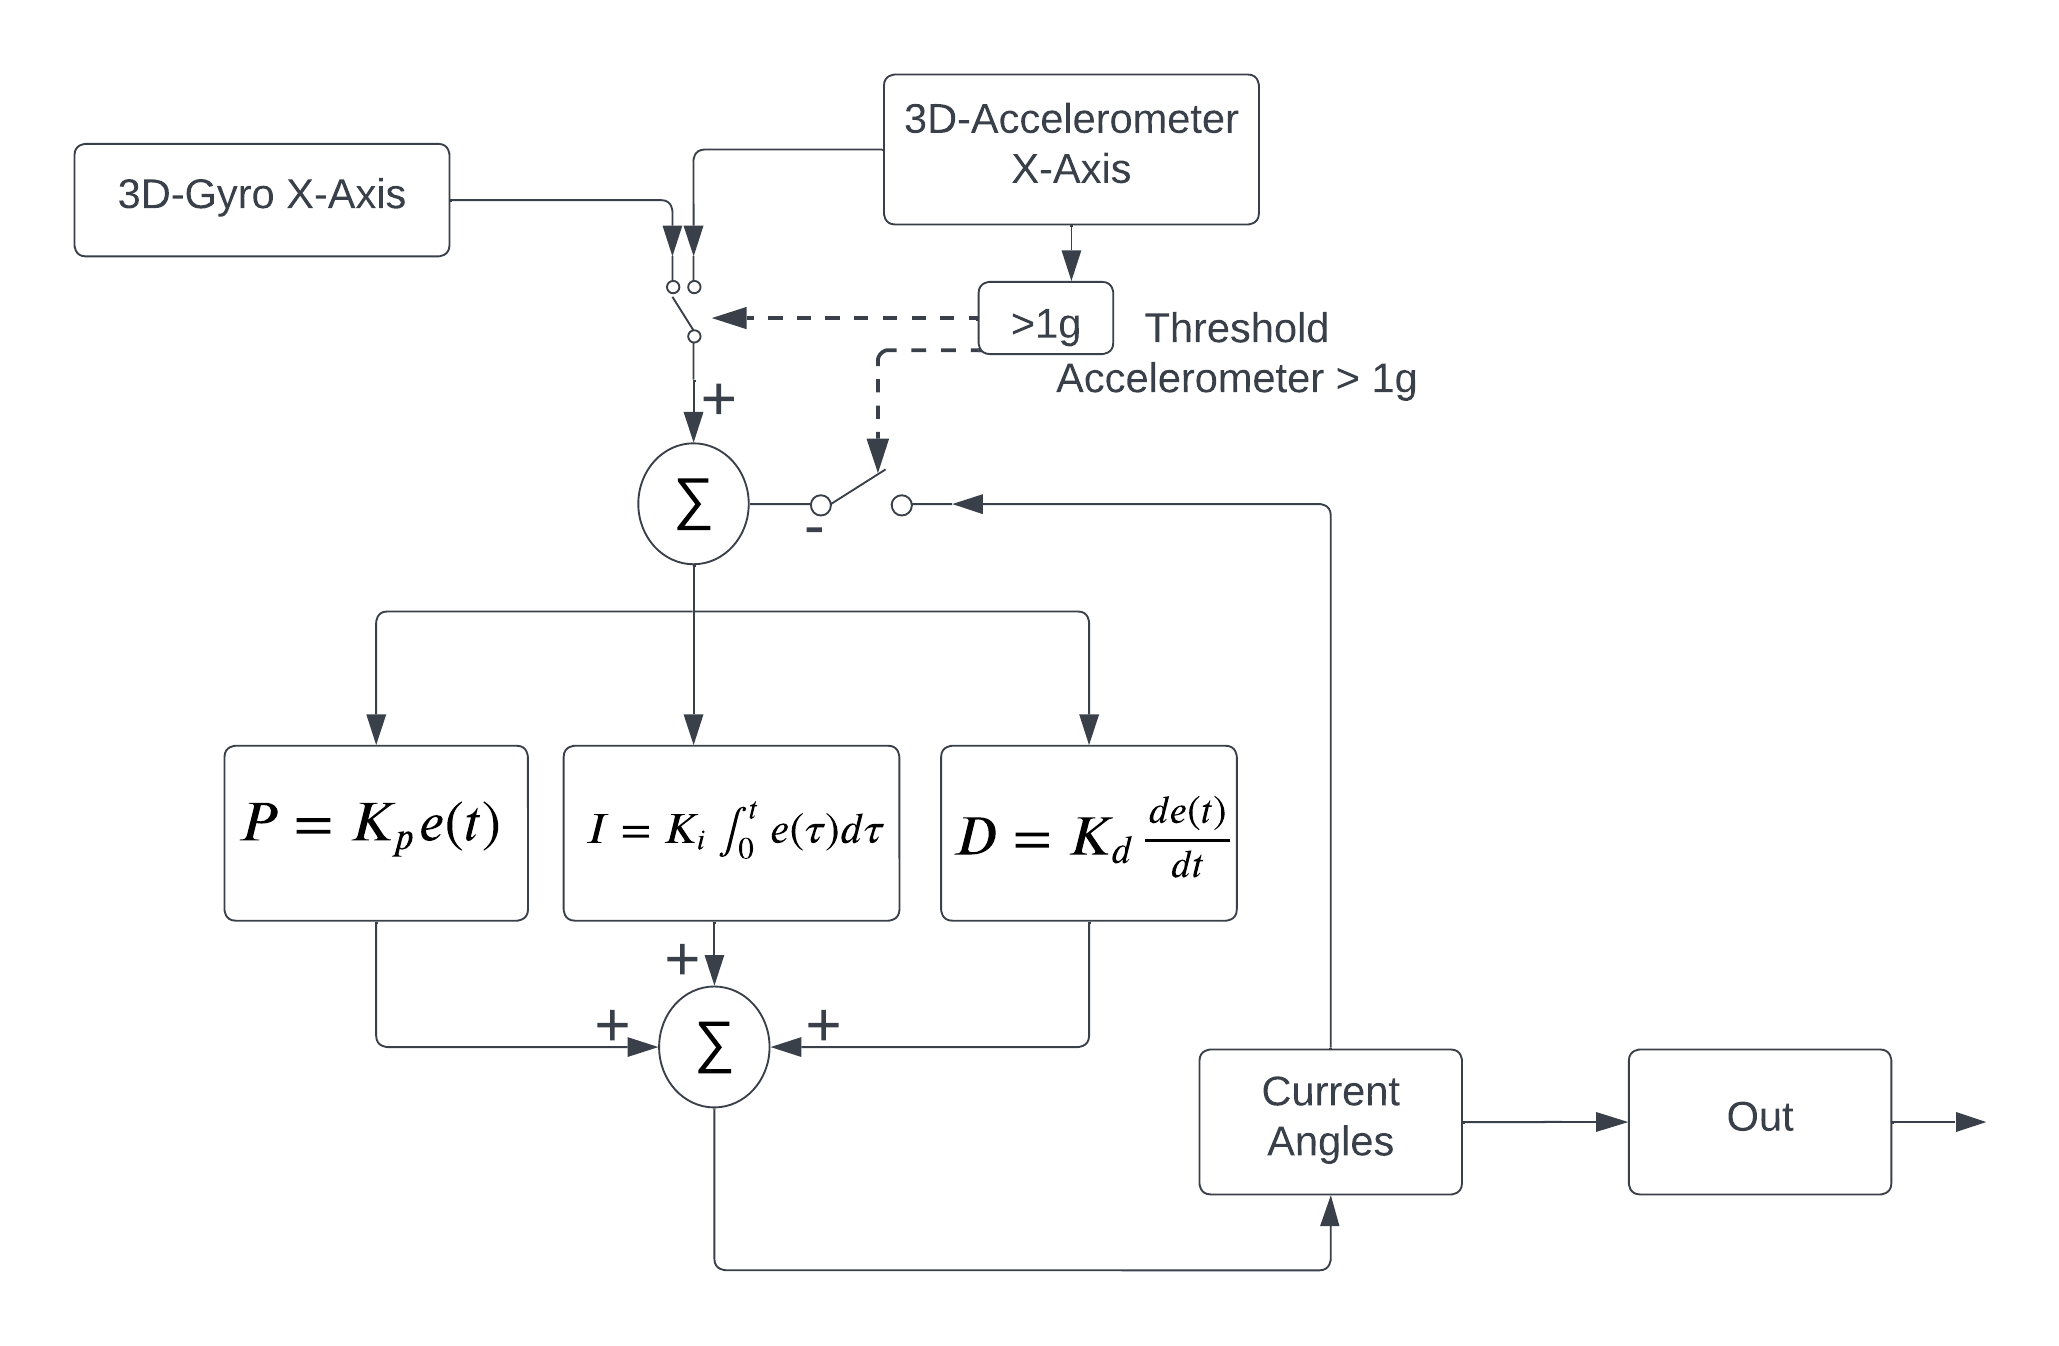
\includegraphics[width=1\linewidth]{content/images/PID_Loop.png}
    \caption{PID Loop}
  \end{center}
\end{figure}

\subsection{UseCase}
\begin{figure}[H]
  \begin{center}
    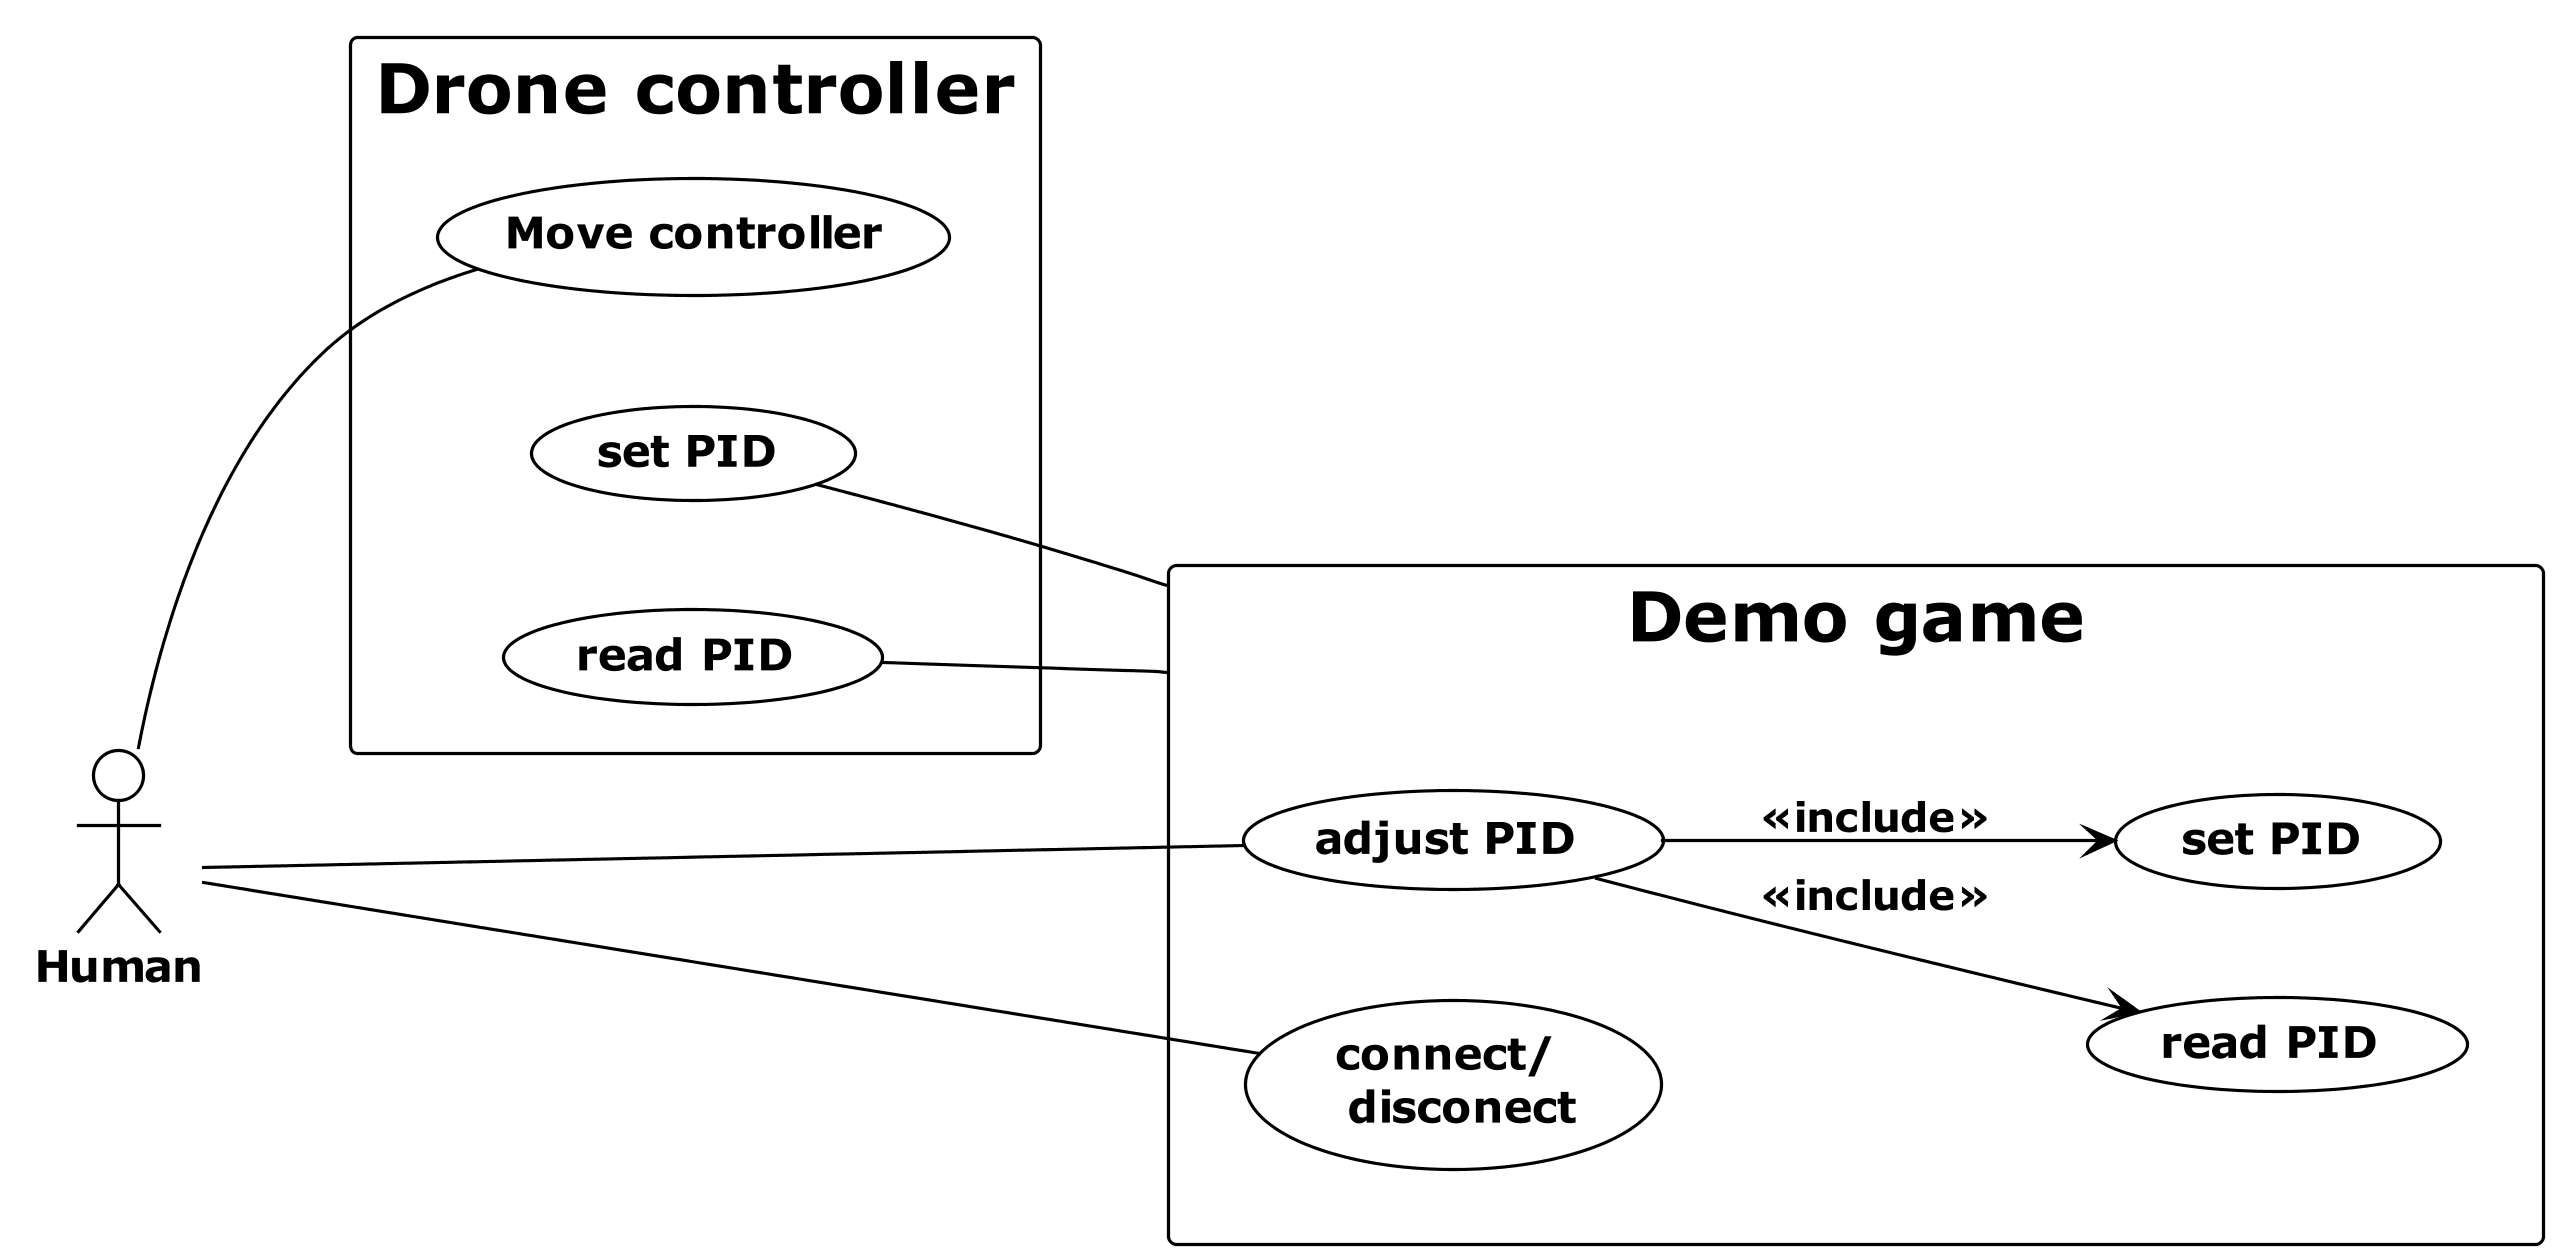
\includegraphics[width=0.8\linewidth]{content/diagrams/out/usecase/sendAngles.png}
    \caption{Send angles}
  \end{center}
\end{figure}

\subsection{Sequenzdiagramme}
\begin{figure}[H]
  \begin{center}
    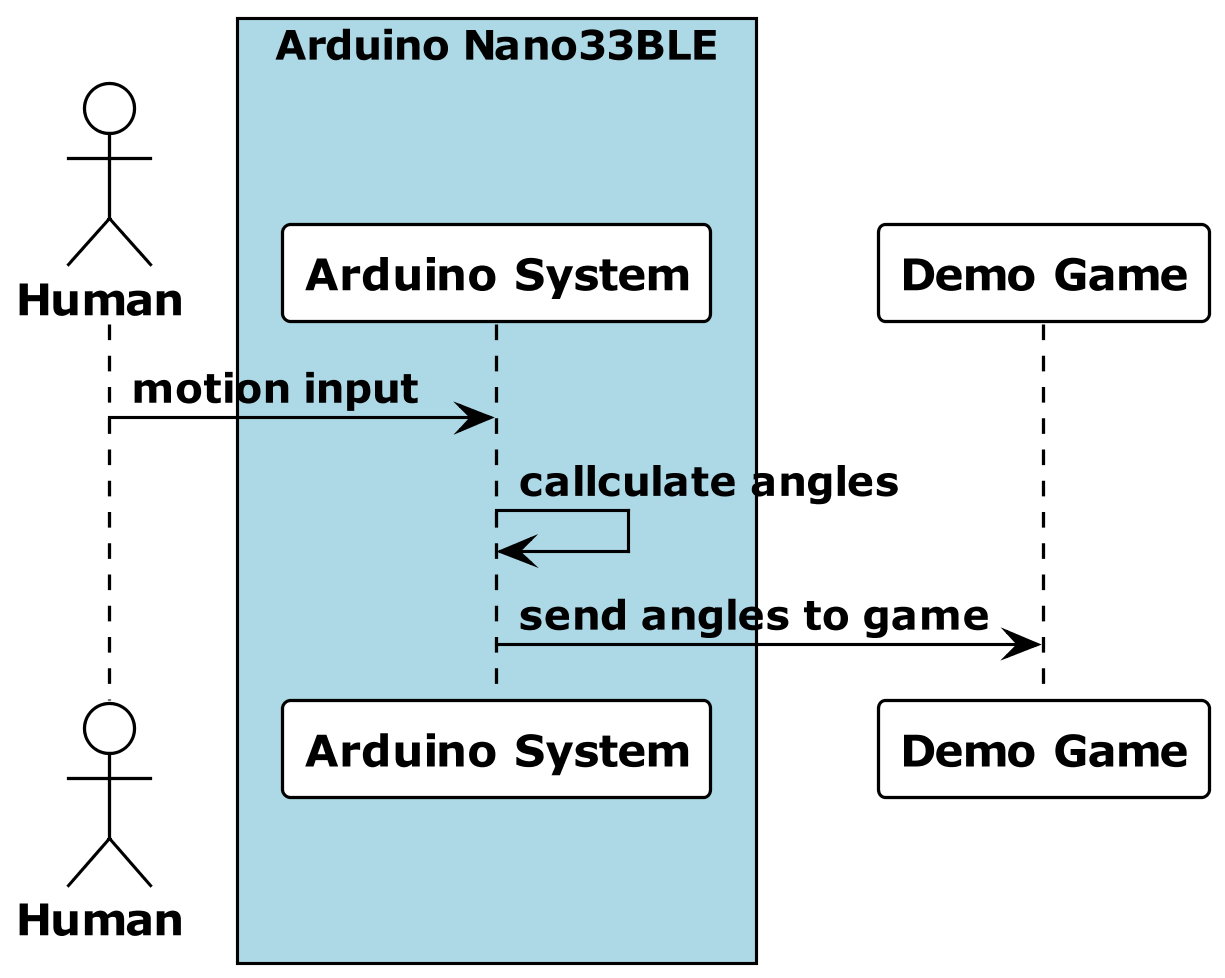
\includegraphics[width=0.7\linewidth]{content/diagrams/out/sequence/system.png}
    \caption{System}
  \end{center}
\end{figure}

\begin{figure}[H]
  \begin{center}
    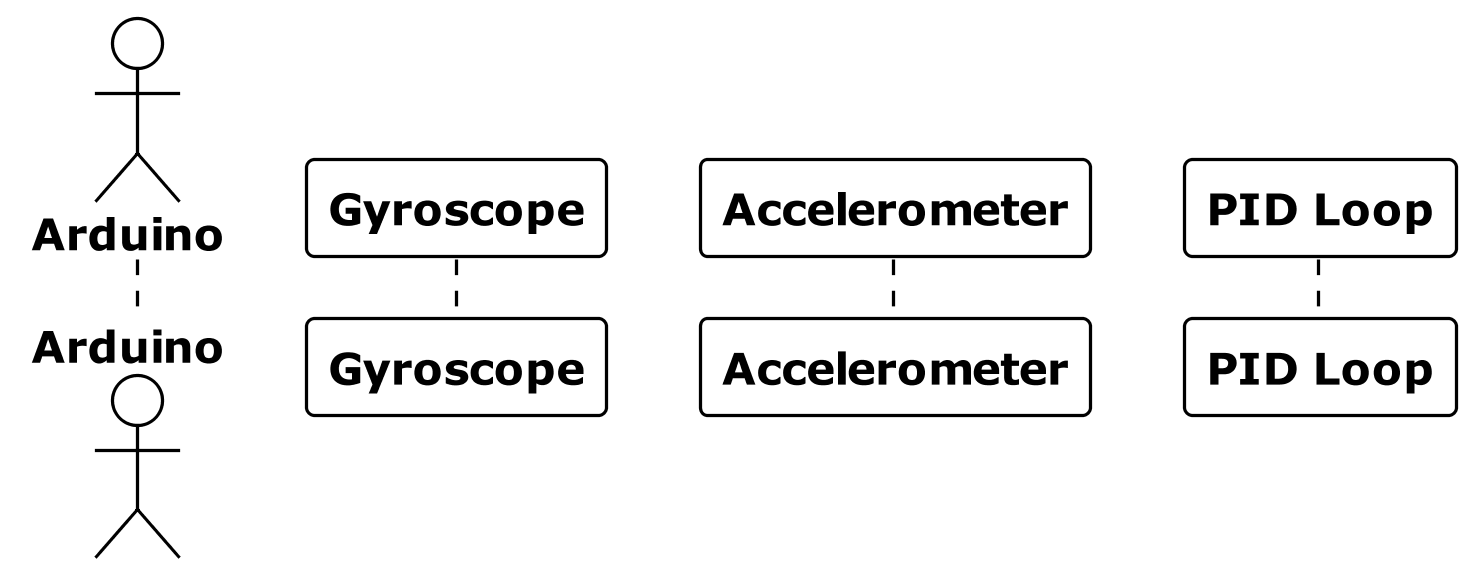
\includegraphics[width=0.8\linewidth]{content/diagrams/out/sequence/arduino.png}
    \caption{Arduino}
  \end{center}
\end{figure}

\begin{figure}[H]
  \begin{center}
    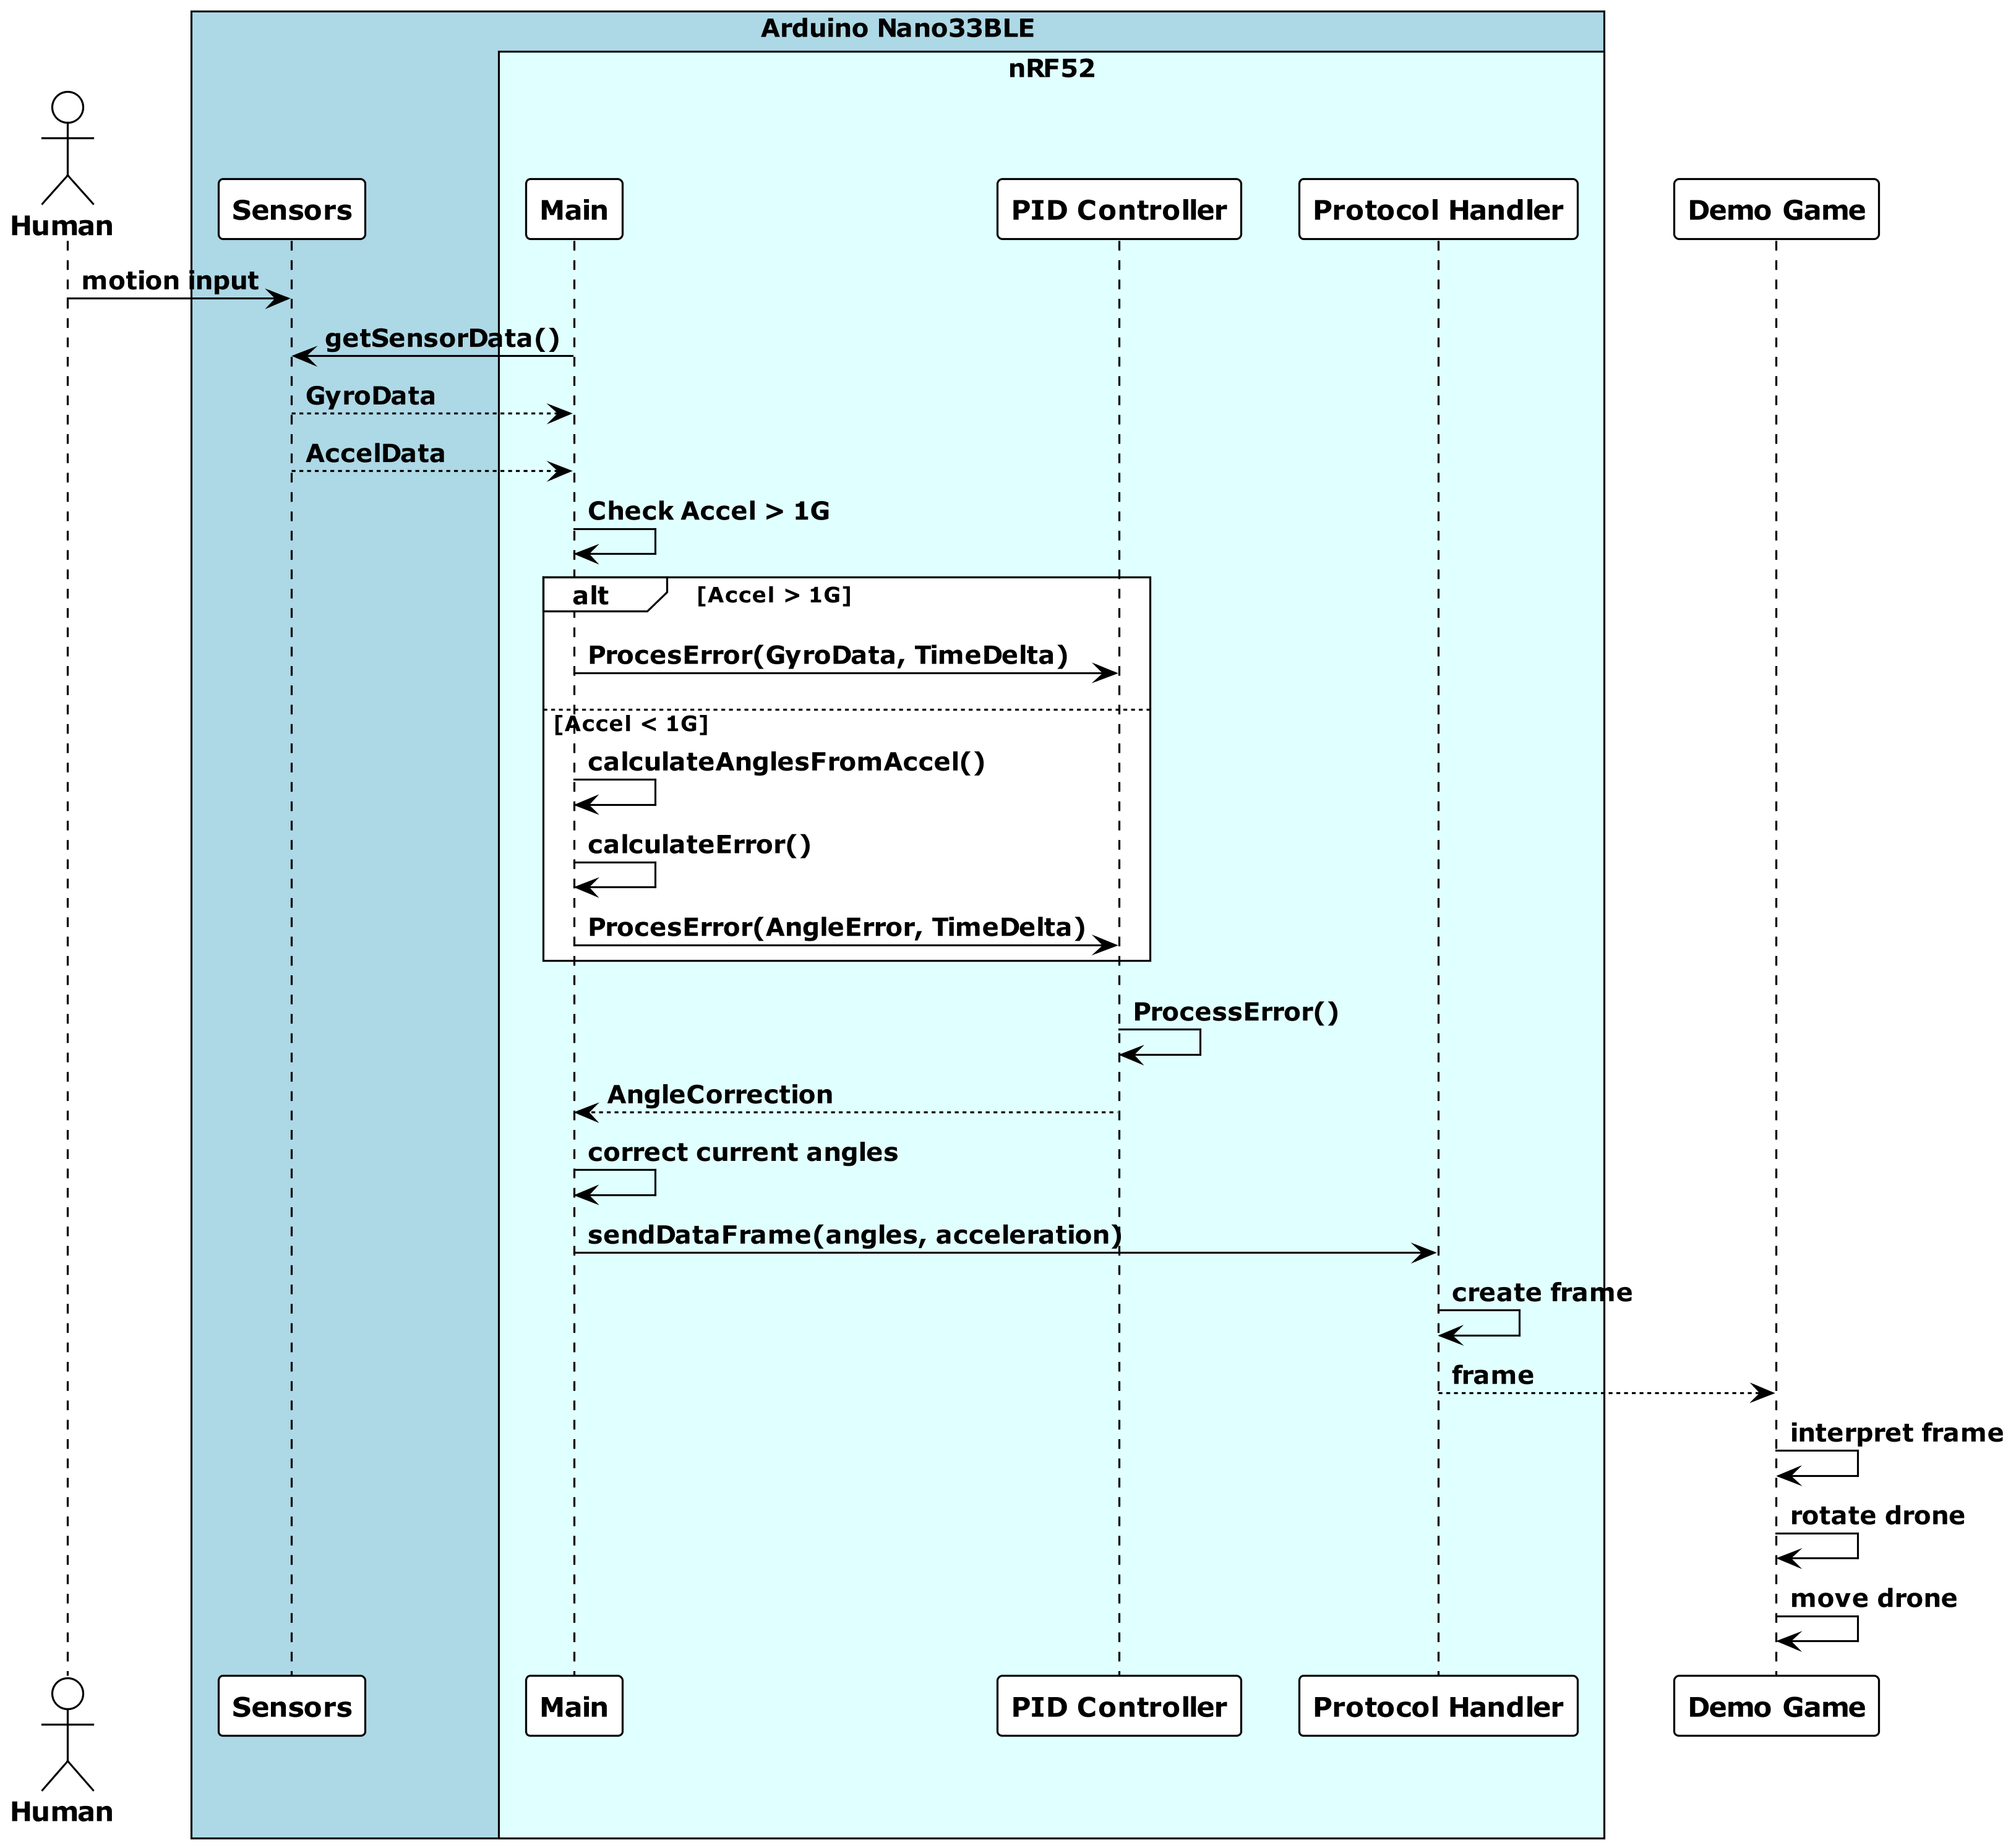
\includegraphics[width=0.8\textheight]{content/diagrams/out/sequence/moveController.png}
    \caption{Move controller}
  \end{center}
\end{figure}


\section{Ablage Dokumentation und Code}
Der gesamte Code und die Dokumentation sind mit GIT über GitHub verwaltet.\\

Der Code kann über diesen Link abgerufen werden:\\
\url{https://github.com/sirtheta/Drohnensteuerung}


% Abbildungsverzeichnis
\newpage 
\pagestyle{plain}
\thispagestyle{empty}
 
\newpage
\pagenumbering{alph}

%\phantomsection \label{listoffig}
\listoffigures
\newpage
\listoftables

% \clearpage
% \bibliographystyle{agsm}
% \bibliography{ArbeitBib}
\end{document}